
\begin{table*}[t]
\centering
\begin{tabular}{c|cc|cc|ccc}
  \specialrule{.2em}{.1em}{.1em}
  \multirow{2}{*}{Module} & \multicolumn{2}{c|}{\multirow{2}{*}{Ablation}} &
  \multicolumn{2}{c|}{K=1} & \multicolumn{3}{c}{K=6} \\
 & & & minADE & minFDE & minADE & minFDE & MR \\
  \hline
  \multirow{7}{*}{LaneRoI Encoder} & \ROI & Shortcut & & & & & \\
  \cline{2-8}
              & & & 1.68 & 3.79 & 0.86 & 1.46 & 14.5 \\
  & \checkmark & & 1.68 & 3.84 & 0.82 & 1.36 & 12.9 \\
  & \checkmark & Global Pool & 1.69 & 3.84 & 0.84 & 1.38 & 12.8 \\
  & \checkmark & Center Pool & 1.67 & 3.80 & 0.83 & 1.35 & 12.4 \\
  & \checkmark & Ours x 1 & 1.55 & 3.45 & 0.81 & \textbf{1.29} & 11.1 \\
  \rowcolor{grey} \cellcolor{white}& \checkmark & Ours x 2 & \textbf{1.54} &
  \textbf{3.45} & \textbf{0.80} & \textbf{1.29} & \textbf{10.8}\\
  \specialrule{.1em}{.05em}{.05em}
  \specialrule{.1em}{.05em}{.05em}
  \multirow{8}{*}{LaneRoI Interactor} & Interactor-Arch & Pooling & & & & & \\
  \cline{2-8}
                              & & & 1.54 & 3.45 & 0.80 & 1.29 & 10.8 \\
  & Attention & Global & 1.42 & 3.10 & 0.78 & 1.24 & 9.8 \\
  & Attention & Shortcut & 1.47 & 3.22 & 0.80 & 1.25 & 10.1 \\
  & GNN & Global & 1.45 & 3.15 & 0.79 & 1.25 & 9.9 \\
  & GNN & Shortcut & 1.45 & 3.21 & 0.79 & 1.25 & 10.0 \\
  & Ours & AvgPool & 1.42 & 3.11 & 0.79 & 1.25 & 9.9 \\
  \rowcolor{grey} \cellcolor{white} & Ours & LanePool & \textbf{1.33} &
  \textbf{2.85} & \textbf{0.77} & \textbf{1.19} & \textbf{8.2}\\
  \specialrule{.1em}{.05em}{.05em}

\end{tabular}
\caption{Ablations on different modules of LaneRCNN. Metrics are reported on the validation set.
In the upper half, we examine our \ROI Encoder, comparing per-actor 1D feature vector 
v.s. \ROI representations as well as different designs for the shortcut mechanism.
In the lower half, we compare different strategies to model interactions, including a
fully connected graph among actors with GNN / attention, as well as ours.
Pooling refers to how we pool a 1D actor feature from each \ROI which are
used by GNN / attention. Rows in gray indicate the architecture used in
our final model.}
\label{table:ablation}
\end{table*}




\section{Experiment}

We evaluate the effectiveness of LaneRCNN on the large-scale Argoverse motion
forecasting benchmark (Argoverse), which is publicly available and provides annotations
of both actor motions and HD maps. In the following, we first
explain our experimental setup and then compare our method against
state-of-the-arts. We also conduct ablation studies on each
module of LaneRCNN to validate our design choices. Finally, we present some
qualitative results.

\subsection{Experimental Settings}
\paragraph{Dataset}
Argoverse provides a large-scale dataset \cite{argoverse} for the
motion forecasting task, which is to
forecast 3 seconds future motions of a particular actor (labeled with type
`agent') given 2 seconds past observations of all
actors in the scene, sampled at 10Hz. 
This dataset consists of more than 30K real-world driving sequences collected in Miami and Pittsburgh.
Those sequences are further split into train, validation, and test sets without
any geographical overlapping. 
% Each of them has 205942, 39472, and 78143 sequences
% respectively. In particular, each sequence contains the positions of all actors in
% a scene within the past 2 seconds history, annotated at 10Hz.
% For each sequence, it specifies one interesting actor in this scene, with type `agent', whose future 3 seconds
% motions are used for the evaluation. 
% The train and validation splits additionally
% provide future locations of all actors within 3 second horizon labeled at 10Hz, while 
Annotations of future timesteps for test sequences are withheld from the public and used for
the leaderboard evaluation. Besides, HD map information can be retrieved for all
sequences. 

\paragraph{Metrics} We follow the benchmark setting and use Miss-Rate (MR), Average
Displacement Error (ADE) and Final Displacement Error (FDE), which are also
widely used in the community. MR is defined as the ratio of data that none of
the predictions has less than 2.0 meters L2 error at the final timestep. ADE is
the averaged L2 errors of all future timesteps, while FDE only
counts the final timestep. To evaluate the mutli-modal prediction, we
also adopt the benchmark setting: predicting K=6 future trajectories
per actor and evaluating the $\text{min}_{K}\text{MR}$, $\text{min}_{K}\text{ADE}$,
$\text{min}_{K}\text{FDE}$ using the trajectory that is closest to the
ground-truth.

\paragraph{Implementation Details}
We train our model on the \emph{train} set with the batch size of 64 and terminate at 30
epochs. We use Adam \cite{adam} optimizer with the learning rate initialized at 0.01 and decayed by 10 at 20 epochs. To normalize the data, we translate and rotate the coordinate system of each sequence so that
the origin is at current position ($t=0$) of `agent' actor and x-axis is aligned
with its current direction. During training, we further apply a random rotation
data augmentation within $(-\frac{2}{3}\pi, \frac{2}{3}\pi)$. No other data
processing is applied such as label smoothing. 
% More implementation details are provided in the supplementary~\ref{sec:supp_implement}.

\subsection{Comparison with State-of-the-art}
We compare our approach to several recent state-of-the-art methods and summarize
their performance on the test set in Table~\ref{table:argo}. Those methods
include: UULM-MRM~\cite{argoleaderboard} (rasterization based model, joint winner
of Argoverse Forecasting Challenge), WIMP~\cite{wimp} (recurrent graph-based
attention model), VectorNet~\cite{vectornet} (lane topology based GNN model),
LaneGCN~\cite{lgn} (lane topology based GCN model),
SAMMP~\cite{mercat2020multi} (self-attention based model, joint winner of
Argoverse Forecasting Challenge) and TNT~\cite{tnt} (target based model built
upon vectornet). Note that all of them largely beat the Argoverse baselines
(NN+Map and LSTM+Map), indicating this is a highly competitive benchmark.
Nevertheless, our method significantly outperform all previous method on the
official ranking metric (MR, K=6), and also beat most of the methods on other
metrics. 
% We compare our approach with top entries on Argoverse motion forecasting
% leaderboard \cite{argoleaderboard} as well as official baselines provided
% by the dataset \cite{argoverse} as shown in Table \ref{table:argo}. 
% We only submit our final model once to the leaderboard and achieve
% state-of-the-art performance.\footnote{Snapshot of the leaderboard at the submission time: Nov. 12, 2020.}
% This is a very challenging benchmark
% with around 100 participants at the time of our submission. Note that for the
% official ranking metric MR (K=6), previous leading methods are extremely close to
% each other, implying the difficulty of further improving the performance.
% Nevertheless, we significantly boost the number which verifies the
% effectiveness of our method. Among the competitors, both Jean
% \cite{mercat2020multi} and TNT \cite{tnt} use RNNs to encode actor kinematic
% states and lane polylines. They then build a fully-connected interaction graph
% among all actors and lanes, and use either the attention or GNNs to model
% interactions. As a result, they represent each actor with a single
% feature vector, which is less expressive than our \ROI representations. Moreover,
% the fully-connected interaction graph may also discard valuable map structure
% information. Note that TNT shares a similar output parameterization as
% ours, yet we perform better on all metrics. This further validates the advantages of
% our \ROI compared against traditional representations. Unfortunately, since Poly team does
% not publish their method, we can not compare with it qualitatively.


\begin{figure*}[t]
\vspace{-0.2cm}
\centering
\setlength{\tabcolsep}{1pt}
\begin{tabular}{cccc}
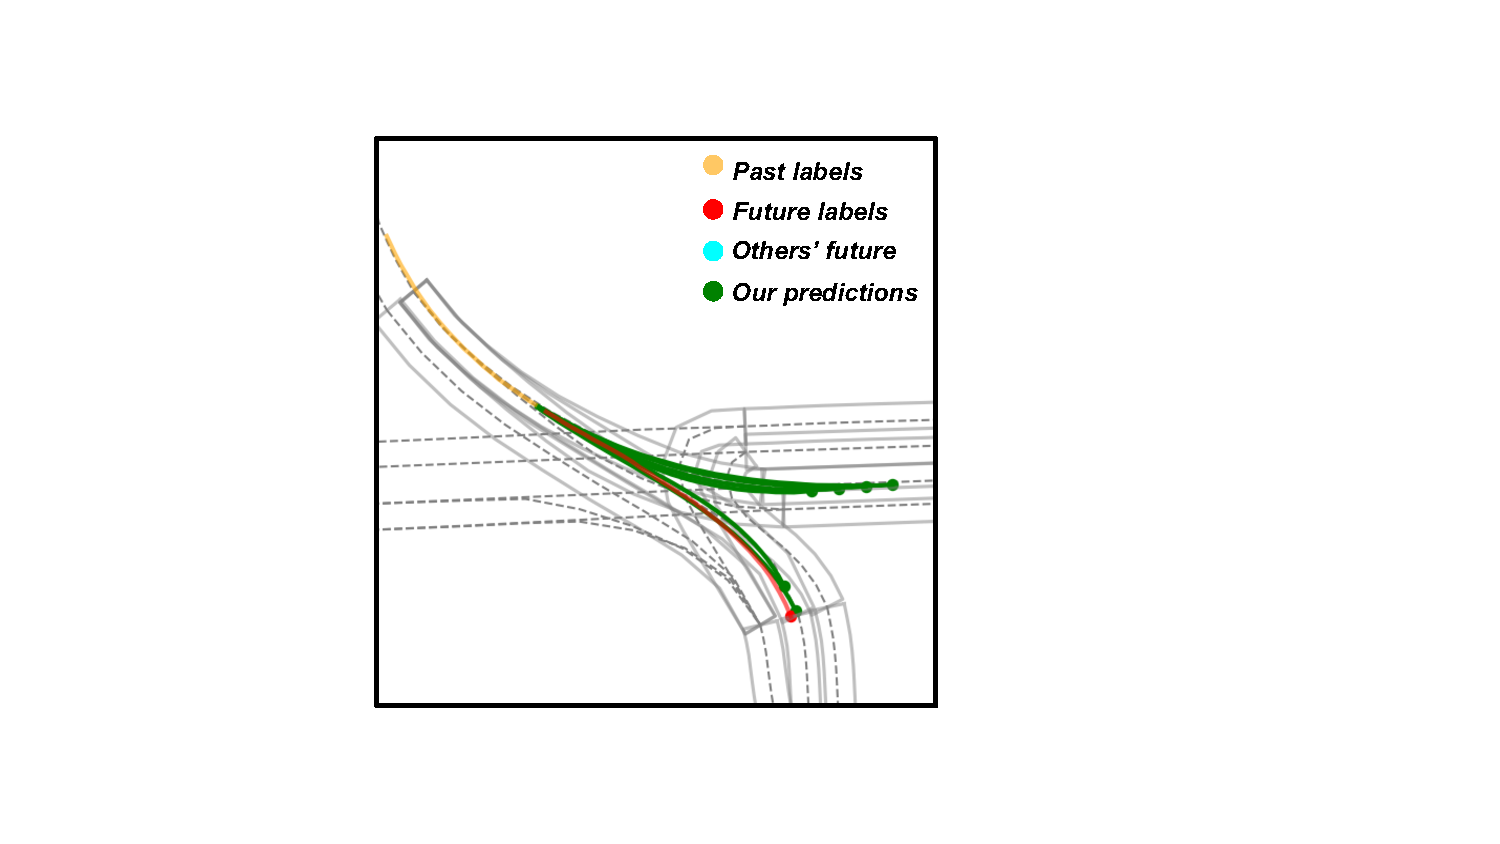
\includegraphics[width=0.24\linewidth]{figures/vis1.pdf}
&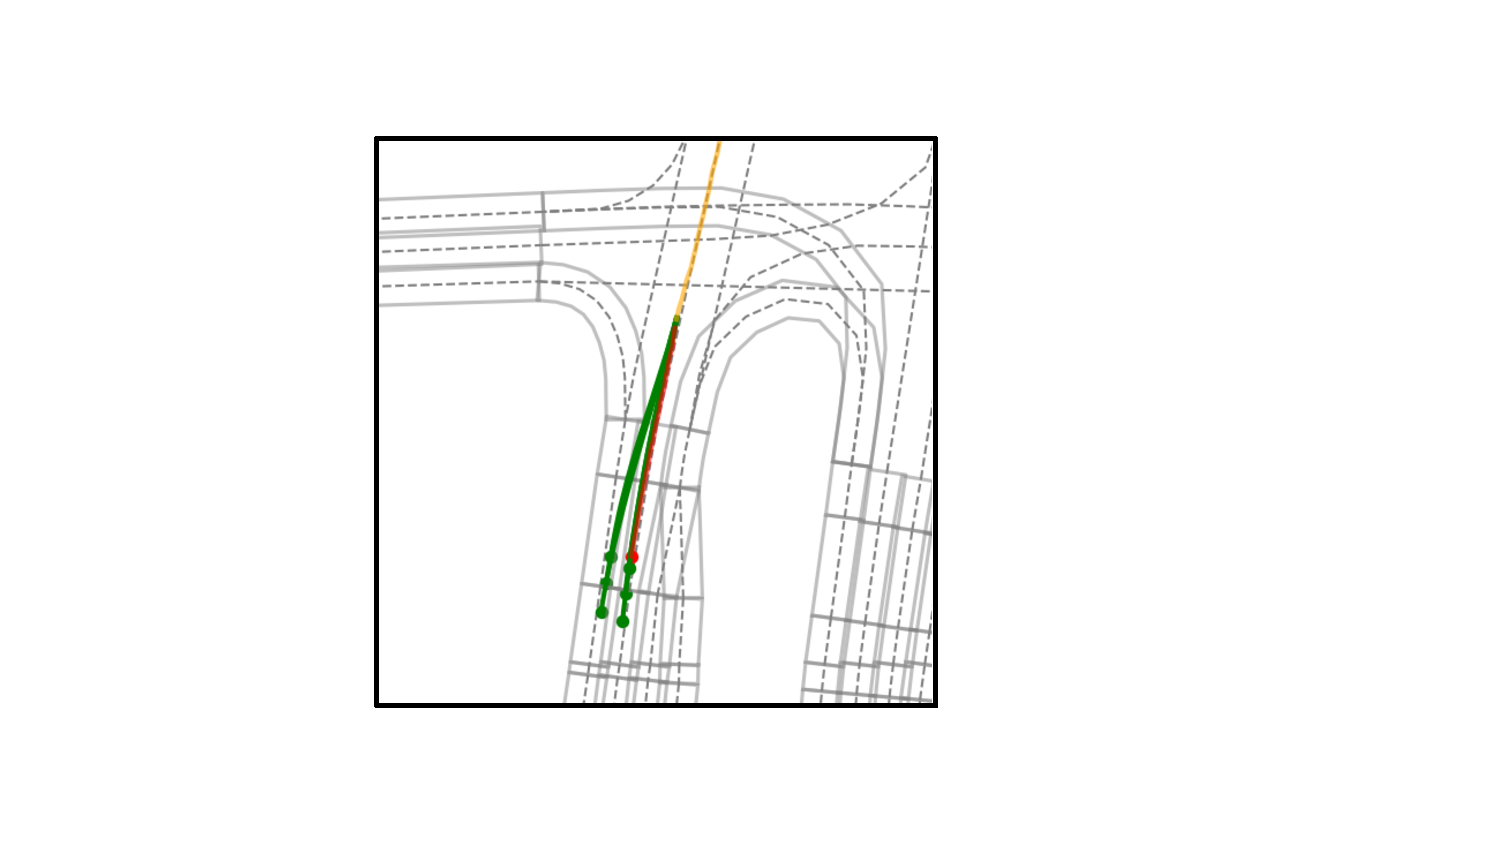
\includegraphics[width=0.24\linewidth]{figures/vis2.pdf}
&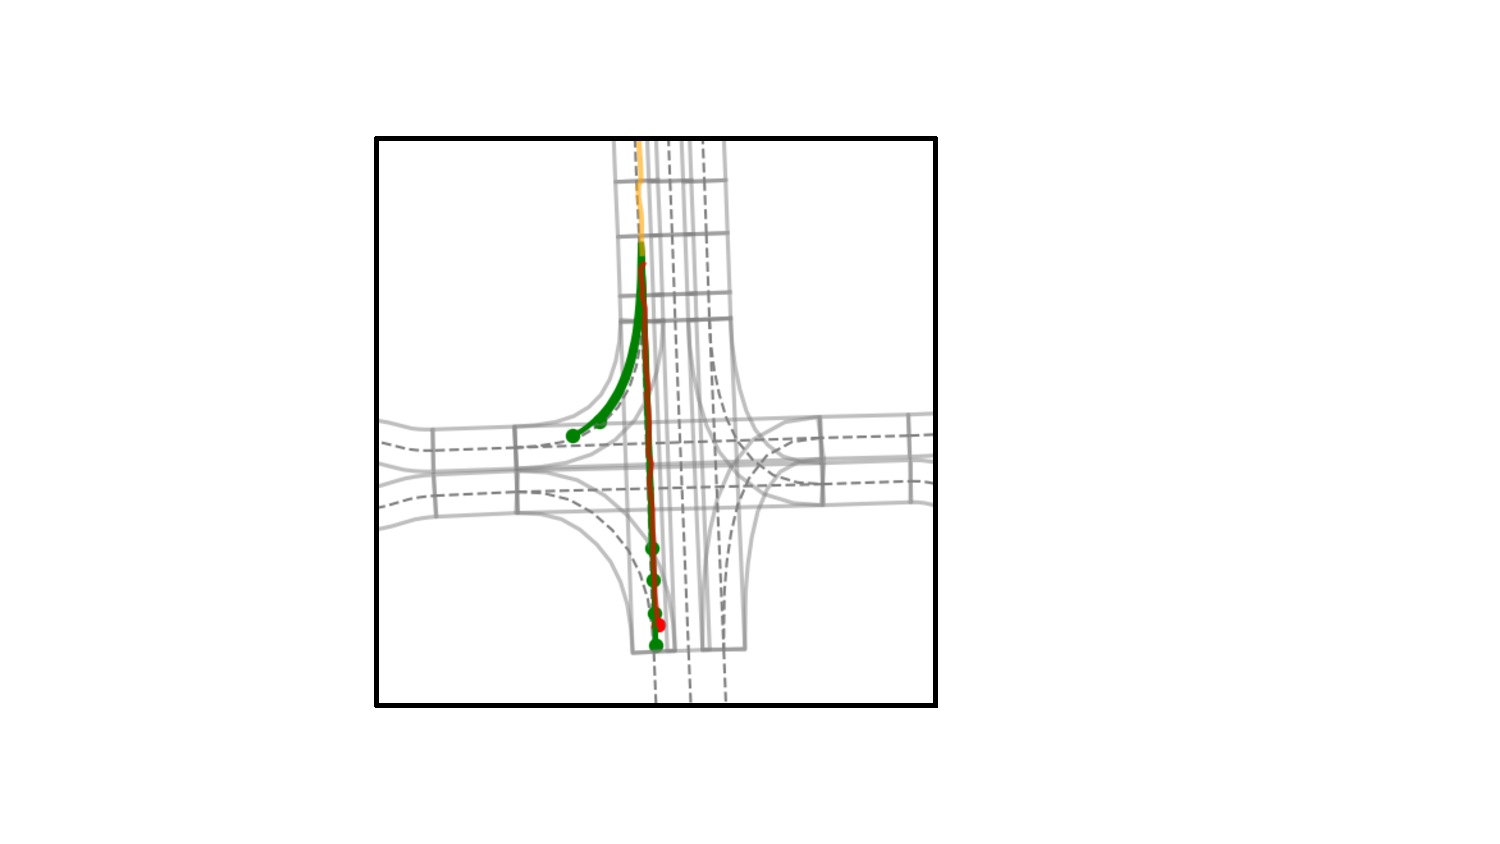
\includegraphics[width=0.24\linewidth]{figures/vis3.pdf}
&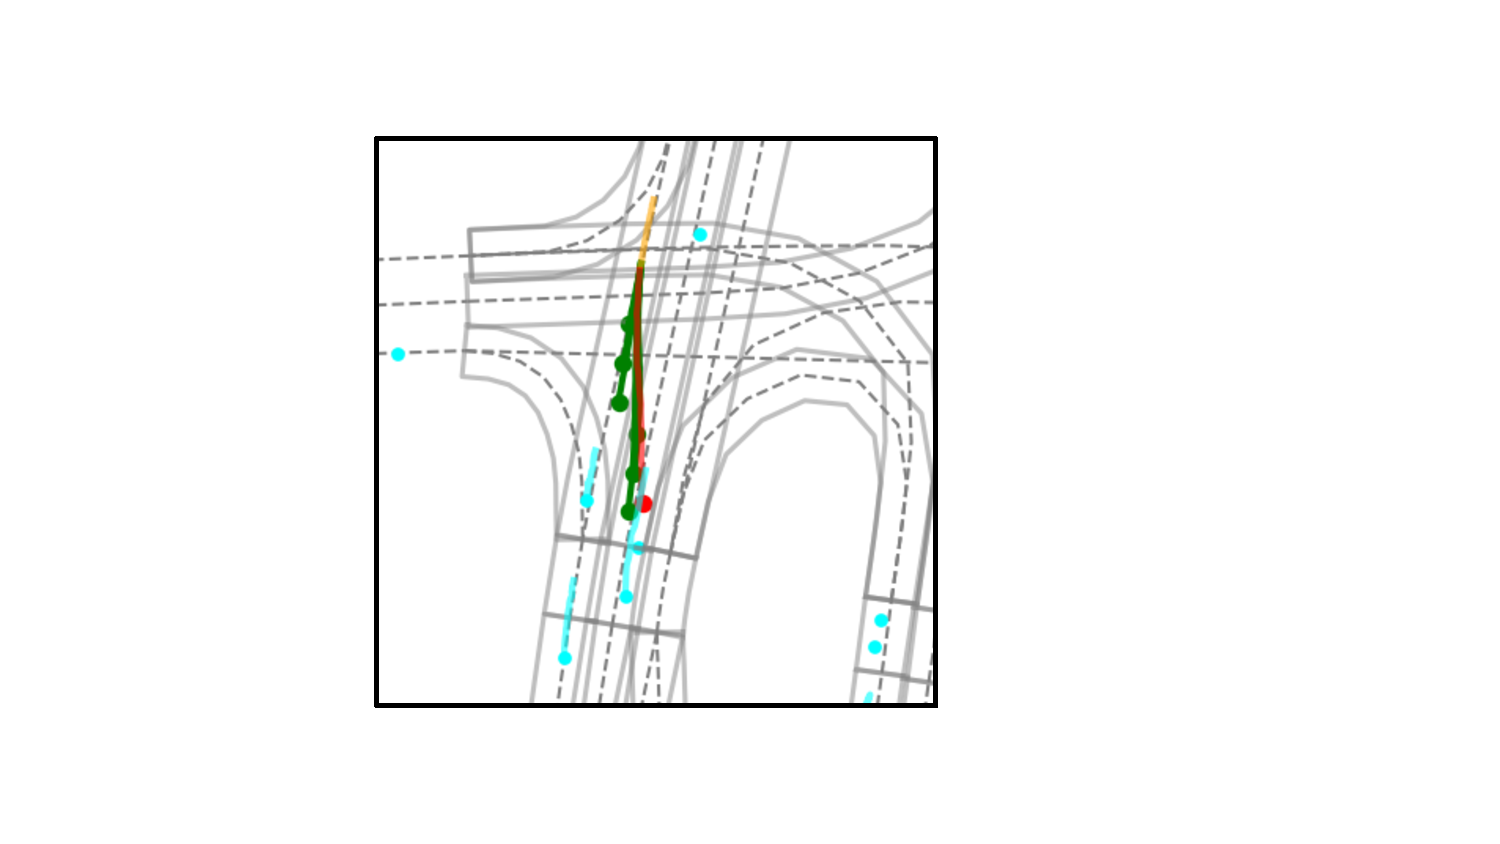
\includegraphics[width=0.24\linewidth]{figures/vis4.pdf}

\end{tabular}
\caption{Qualitative results on Argoverse validation set. Here we show (from
left-to-right): 1) curved lanes 2) lane changing 3) intersection 4) overtaking.}
\label{fig:vis}
\vspace{-0.2cm}
\end{figure*}

\subsection{Ablation Studies}





\paragraph{Ablations on LaneRoI Encoder}
We first show the ablation study on one of our main contributions, \ie, \ROI, in the upper half of Table
\ref{table:ablation}. 
The first row shows a representative of the traditional representations. 
Specifically, we first build
embeddings for lane graph nodes using only the map information and 4 lane
convolution layers. We then use a
1D CNN (U-net style) to extract a motion feature vector from actor kinematic states, concatenate it
with every graph node embedding and make predictions. Conceptually, this is
similar to TNT \cite{tnt} except that we modify the backbone network to make comparisons fair. 
On the second row, we show the result of our \ROI
representations with again four lane convolution layers (no shortcuts). Hence, the only difference
is whether the actor is encoded with a single motion vector shared by
all nodes, or encoded in a distributed and structured manner as ours. As shown
in the table, our \ROI achieves similar or better results on all
metrics, exhibiting its advantages. Note that this row is not yet our best result
in terms of using \ROI representations, as the actor information is only exposed
to a small region during the input encoding (clamping at input
node embeddings) and can not efficiently propagate to
the full \ROI without the help of the shortcut, which we will show next.

Subsequent rows in Table \ref{table:ablation} compare different design
choices for the shortcut mechanism, in particular how we pool the global feature
for each \textit{LaneRoI}. `Global Pool' refers to average-pooling all node
embeddings within a \textit{LaneRoI}, and `Center Pool' means we pool a feature
from a \ROI using nodes that around the last observation of the actor and a lane
pooling. As we can see, although these two approaches can possibly
spread out information to every node in a \textit{LaneRoI} (and thus build a
shortcut), they barely improve the performance. On the contrary, ours achieve
significant improvements. This is because we pool features along the past
trajectory of the actor, which results in a larger and actor-motion-specific receptive field.
Here, $\times 1$ and $\times 2$ refer to an encoder with 1 shortcut per 4 and 2 lane
convolution layers respectively. This shows stacking more shortcuts
provides some, but diminishing, benefits.









\paragraph{Ablations on LaneRoI Interactor}
To verify the effectiveness of our map-aware interaction module, we compare against several model variants based
on the fully-connected interaction graph among actors. Specifically, for each actor,
we apply a \ROI encoder\footnote{We choose \ROI encoder rather than other
encoder, \eg, CNN, for fair comparisons with ours.} to process node embeddings, and then pool an
actor-specific feature vector from \ROI via either the global average pooling or our
shortcut mechanism. These actor features are then fed into a transformer-style
\cite{transformer} attention module or a fully-connected GNN.
Finally, we add the output actor features to nodes in their \ROI respectively
and make predictions using our decoding module.
As a result, these variants have the same pipeline as ours, with the only
difference on how to communicate across actors. To make comparisons
as fair as possible, both the attention and GNN have the same
numbers of layers and channels as our \ROI Interactor.\footnote{The GNN here is almost identical to our lane
convolution used in Interactor except for removing the multi-hop as the graph is fully-connected.}

As shown in Table \ref{table:ablation}, all interaction-based models outperform
the one without considering interactions (row 1) as expected. In addition, our
approach significantly improves the performance compared to both the attention and GNN. 
Interestingly, all fully-connected interaction graph based model reach similar
performance, which might imply such backbones may saturate the performance (as
also shown by leading methods on the leaderboard).
We also show that naively using the average pooling to embed features from
\textit{LaneRoI}s to global graph does not achieves good performance
because it ignores local structures.

\subsection{Qualitative results}
In Figure~\ref{fig:vis}, we show some qualitative results on Argoverse validation
set. We can see that our method generally follows the map very well and demonstrates good
multi-modalities. From left to right, we show 1) when an actor follows a
curved lane, we predict two direction modes with different velocities;
2) when it is on a straight lane, our model covers the possibilities of lane changing; 3)
when it's approaching an intersection, our model captures both the go-straight and the
turn-right modes, especially with lower speeds for turning right, which are
quite common in the real world; 4) when there is an actor blocking the path, we
predict overtaking behaviors matching exactly with the ground-truth. Moreover,
for the lane-following mode, we predict much slower speeds which are consistent with
this scenario, showing the effectiveness of our interaction modeling. 
% We provide more qualitative results in the supplementary~\ref{sec:supp_qual}.

